\documentclass[12]{beamer}

\usepackage[russian]{babel}
\usepackage{tikz}


\usetheme[progressbar=frametitle]{metropolis}
\setbeamertemplate{frame numbering}[fraction]
\usefonttheme{metropolis}
\setbeamercolor{background canvas}{bg=white}


\title{Семинары 4 и 5}
\subtitle{Уравнение Шредингера. Ямы и Барьеры.}
\author{}
\date{\today}
\institute {\large 
\textbf{Ключевые слова}: Волновая функция, операторы физических величин, уравнение Шредингера, туннельный эффект, потенциальные ямы\\[6pt] 

\\[6pt] 
\textbf{Задачи}: 3.4, 3.34, 3.40, 3.14\\[6pt] 

}


\begin{document}
\metroset{block=fill}
\maketitle


\begin{frame}[t]{Волновая функция}
Импульс частицы и ее длина волны $p  = \hbar k = \dfrac{h}{\lambda}$\\
Энергия частицы и частота: $E  = \hbar \omega$
\begin{block}{Волновая функция}
\begin{equation*}
    \psi = \psi_0 \exp{\left[i\left(kx - \omega t \right)\right]} =\psi_0 \exp{\left[\dfrac{i}{\hbar}\left(px - Et \right)\right]}
\end{equation*}
\end{block}
\begin{block}{Свойства $\psi$-функции}
\begin{itemize}
    \item Непрерывность
    \item Гладкость
    \item Нормировка: $\int\psi^*\psi dV = 1$
\end{itemize}
\end{block}
\begin{block}{Принцип суперпозиции}
$\psi = c_1\psi_1 + c_2\psi_2 \Rightarrow \psi^*\psi = c^2_1\psi^2_1 + c^2_2\psi^2_2; \psi^*_1\psi_2=\psi^*_2\psi_1=0 $
\end{block}

\end{frame}

\begin{frame}[t]{Операторы}

\begin{block}{Классика}
Обычные функции: $ \textbf{r}_1 \rightarrow \textbf{r}(t)  \rightarrow \textbf{r}_2$
\end{block}

\begin{block}{Кванты}
Функции над функциями (операторы): $ \psi_1(\textbf{r}, t) \rightarrow \hat{F(\textbf{r},t)}  \rightarrow \psi_2(\textbf{r}, t)$
\end{block}
\begin{block}{Свойства операторов}
\begin{itemize}
    \item Линейность
    \item Связь оператора с физической величиной через собственные значения
\end{itemize}
\end{block}
\end{frame}

\begin{frame}[t]{Операторы}
\begin{block}{Координата}
\begin{equation*}
    \hat{x}\psi = x\psi
\end{equation*}
\end{block}

\begin{block}{Импульс}
\begin{gather*}
    \hat{p_x}\psi = -i\hbar\dfrac{\partial\psi}{\partial x} = p_x \psi\\
    \hat{\textbf{p}}\psi = -i\hbar\nabla\psi = \textbf{p} \psi
\end{gather*}
\end{block}

\begin{block}{Энергия (оператор Гамильтона)}
\begin{equation*}
    \hat{H}\psi = \hat{T}\psi + \hat{U}\psi = \dfrac{\hat{p}^2}{2m}\psi + \hat{U}\psi  = -\hbar^2\Delta\psi + U(x,y,z)\psi
\end{equation*}
\end{block}

\end{frame}

\begin{frame}[t]{Уравнение Шредингера}
\begin{block}{Стационарное}
\begin{equation*}
    \hat{H}\psi = E\psi
\end{equation*}
\end{block}

\begin{block}{Нестационарное}
\begin{gather*}
    i\hbar\dfrac{\partial\psi}{\partial t} = \hat{H}\psi
\end{gather*}
\end{block}

\begin{block}{Среднее значение оператора}
\begin{equation*}
    \langle A\rangle = \int\psi^*\hat{A}\psi dV
\end{equation*}
\end{block}

\end{frame}


\begin{frame}[t]{Барьеры и ямы}
Тут мы обратимся к конспекту
\end{frame}




\begin{frame}{Задача 3.4}\scriptsize
\only<1>{\begin{block}{Условие}
Волновая функция частицы массой $m$, совершающей одномерное движение в поле с потенциалом $U(x)$, есть 
\begin{gather*}
\psi(x) = 
    \begin{cases}
        Ax\exp{\left( -\dfrac{x}{a}\right)}; &x \ge 0\\
        0; &x<0
    \end{cases}
\end{gather*}
Оценить с помощью соотношения неопределенностей среднюю кинетическую энергию $\langle T \rangle$ частицы и сравнить с результатом точного расчета. Найти среднее значение координаты $\langle x \rangle$, а также $U(x)$ при $x>0$ и полную энергию $E$, если известно, что $U(x) \rightarrow 0$ при $x \rightarrow \infty$
\end{block}}
\only<2>{\begin{block}{Решение}
Плотность вероятности найти частицу:
\begin{gather*}
    w(x) = \psi^*\psi = A^2x^2\exp{\left( -\dfrac{2x}{a}\right)} \text{ при }  x \ge 0
\end{gather*}
Найдем максимум:
\begin{gather*}
    \dfrac{dw(x)}{dx} = 0 \Rightarrow x_m = a
\end{gather*}
Тогда неопределенность по координате как $2a$ -- влево и вправо от максимума. Тогда из соотношения неопределенностей:
\begin{gather*}
    p \approx \Delta p = \dfrac{\hbar}{2a} \Rightarrow \langle T \rangle = \dfrac{p^2}{2m} = \dfrac{\hbar^2}{8ma^2}
\end{gather*}
\end{block}
}

\only<3>{\begin{block}{Решение}
Теперь найдем среднее значение координаты честно:
\begin{gather*}
    \langle x \rangle = \dfrac{\int\limits_0^{\infty}\psi(x)^*x\psi(x)dx}{\int\limits_0^{\infty}\psi(x)^*\psi(x)dx} = \dfrac{3a}{2}
\end{gather*}
Подствим в уравнение Шредингера исходную функцию:
\begin{gather*}
    \dfrac{\hbar^2}{2m}\dfrac{\partial^2\psi}{\partial x^2} +  (E-U(x))\psi=0\\
    U(x) - E = \dfrac{\hbar}{2max}\left( \dfrac{x}{a} - 2 \right)
\end{gather*}
Из условия что на бесконечности потенциал равен нулю находим энергию и потенциал:
\begin{gather*}
    E = -\dfrac{\hbar^2}{2ma^2}\\
    U(x) = - \dfrac{\hbar^}{max}
\end{gather*}
\end{block}}
\end{frame}

\begin{frame}{Задача 3.34}\scriptsize
\only<1>{\begin{block}{Условие}
Электрон находится в основном состоянии в одномерной потенциальной яме и имеет энергию $E = 1.5$ эВ. Ширина ямы равна $9a = 3 \cdot 10^{−8}$ см. Найти высоту потенциального барьера $U$ и его проницаемость $D$. За какое время $\tau$ вероятность найти частицу в яме уменьшится в два раза? Отражением волновой функции на задней границе потенциального барьера пренебречь.
\begin{figure}[h]
    \centering
    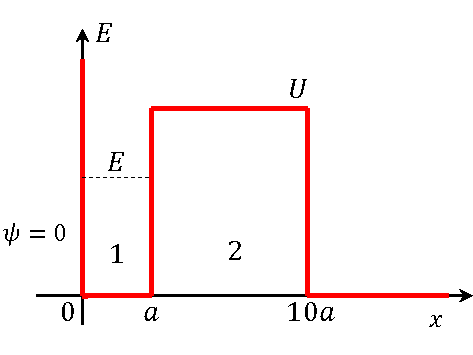
\includegraphics[width=0.6\textwidth,height=\textheight,keepaspectratio]{Seminar_04/pics/pic_05.pdf}

\end{figure}
\end{block}}
\only<2>{\begin{block}{Решение}
апишем уравнение Шредингера в областях 1 и 2:
\begin{gather*}
    \begin{cases}
         \dfrac{\hbar^2}{2m}\dfrac{\partial^2\psi_1}{\partial x^2} +  E\psi_1=0; &a>x>0  \\[10pt]
         \dfrac{\hbar^2}{2m}\dfrac{\partial^2\psi_2}{\partial x^2} - (U - E)\psi_2=0; & 10a>x>a
    \end{cases}
\end{gather*}
Как и раньше обозначим $k = \sqrt{\dfrac{2mE}{\hbar^2}}$ и $ \kappa = \sqrt{\dfrac{2m(U -E)}{\hbar^2}}$. \\Учитывая отсутствие отражения от стенки $10a$, растущей экспоненты во 2 области не будет:
\begin{gather*}
    \begin{cases}
         \psi_1(x) = A \sin{kx} + B \cos{kx}\\
         \psi_2(x) = Ce^{-\kappa x} 
    \end{cases}
\end{gather*}
\end{block}}
\only<3>{\begin{block}{Решение}
Первое: в нуле бесконечная стенка, за ней волновая функция ноль, сшивка только по непрерывности. Отсюда сразу понятно, что $B=0$, так косинус в $x=0$ не 0. Второе: непрерывность в $x=a$. Третье: гладкость там же:
\begin{gather*}
    \begin{cases}
         A \sin{ka} = Ce^{-\kappa a} \\
         Ak \cos{ka} = -C\kappa e^{-\kappa a}
    \end{cases}
\end{gather*}
Отсюда вытащим тангенс и попытаемся через него выразить высоту барьера:
\begin{gather*}
    \tan{ka} = -\dfrac{k}{\kappa}= - \sqrt{\dfrac{E}{U-E}} \Rightarrow U-E = \dfrac{E}{\tan^2{ka}} \Rightarrow U = E(1 + \dfrac{1}{\tan^2{ka}}) = \dfrac{E}{\sin^2{ka}}
\end{gather*}
Окончательно $U = 1.64$ эВ. Проницаемость барьера: $\kappa =1.92\cdot 10^7 \text{ см}^{-1}$,  $D = \exp{\left( -2\kappa(10a-a)\right)} = 3.2\cdot10^{-5}$.
Время уменьшения концентрации частиц вдвое $n=\dfrac{v}{2a}$ -- частота ударов о стенку, тогда:
\begin{gather*}
    (1-D)^{n\tau} = \dfrac{1}{2}\\
    \tau = \dfrac{\ln{2}}{nD} = 1.8\cdot 10^{-11} \text{ c}
\end{gather*}

\end{block}}

\end{frame}

\begin{frame}{Задача 3.40}\scriptsize
\only<1>{\begin{block}{Условие}
В 1988 г. появилось сенсационное сообщение об осуществлении холодного ядерного синтеза дейтерия, растворенного в металлическом палладии. Можно считать, что при этом ядра дейтерия взаимодействуют друг с другом по закону Кулона, если расстояние между ними $r$ удовлетворяет условию $R_1 = 2\cdot 10^{-13} \text{ см} \le r \le  R_2 = 5\cdot 10^{-9} \text{ см}$. При большем расстоянии между ядрами энергия электрического отталкивания $U=0$ за счет экранирования ядер дейтерия электронами проводимости. Определить вероятность реакции синтеза $d+d$ при столкновении дейтронов внутри палладия при комнатной температуре за счет туннельного эффекта. Считать, что реакция синтеза происходит при $r<R_1$.
\begin{figure}[h]
    \centering
    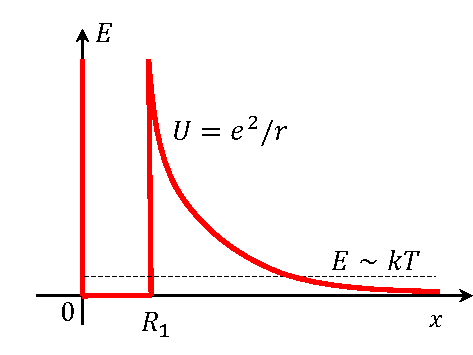
\includegraphics[width=0.4\textwidth,height=\textheight,keepaspectratio]{Seminar_04/pics/pic_06.pdf}

\end{figure}
\end{block}}
\only<2>{\begin{block}{Решение}
Энергия частицы это $E = kT$, для комнатной температуры. Потенциал $U(r) = \dfrac{e^2}{r}$, обычный кулоновский потенциал. Границы интегрирования, это те места где $E=U(r)$, причем из-за малость $R_1$ мы вообще можем забить на нее и сказать, что это 0. Теперь найдем $R_2' = \dfrac{e^2}{kT} \approx 10^{-6} \text{ см}$, Это означает что кинетическая энергия частицы настолько мала, что на придется в качестве верхнего предела брать именно $R_2$ из условия. 
\begin{gather*}
     D  = \exp{\left( -2\int\limits_{0}^{R_2}\sqrt{\dfrac{2m(e^2/r-kT)}{\hbar^2}} dr \right)} = \exp{\left( -\dfrac{2e}{\hbar}\sqrt{2mR_2} \right)} \approx e^{-235} \approx 0
\end{gather*}
\end{block}}
\end{frame}

\begin{frame}{Задача 3.14}\scriptsize
\only<1>{\begin{block}{Условие}
Поток нейтронов падает на длинную щель с абсолютно отражающими стенками. При какой минимальной скорости нейтроны смогут пройти через эту щель?
\begin{figure}[h]
    \centering
    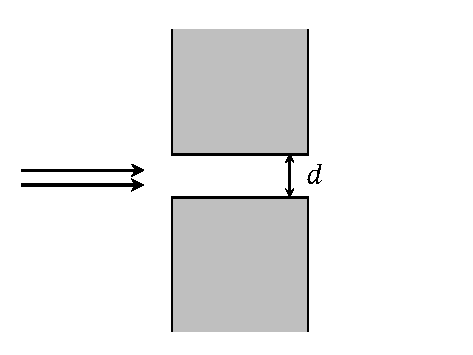
\includegraphics[width=0.3\textwidth,height=\textheight,keepaspectratio]{Seminar_04/pics/pic_07.pdf}
\end{figure}
\end{block}}
\only<2>{\begin{block}{Решение}
Щель для нейтронов выступает в роли ямы с бесконечными стенками. Следовательно, для нейтрона возникают уровни энергий. Следовательно, если энергия нейтрона равна энергиям этих уровней, то нейтрон в щель войдет, и там навсегда останется. То есть у него компонента скорости вдоль начального направления будет нулевая. Если энергия больше, то нейтрон пройдет через эту щель:
\begin{gather*}
    \dfrac{mv^2}{2} > E_{n=1} = \dfrac{\pi^2\hbar^2}{2md^2}
\end{gather*}
\end{block}}
\end{frame}




\begin{frame}[t]{Комментарии к задачам из задания}\scriptsize
\begin{itemize}
\item{Нулевки 4 недели} Задачки на подстановку в формулы из теории
\item{Нулевки 5 недели} Задачки на формулу для энергии частицы в яме с бесконечными стенками
\item{Задача 3.5} Записать уравнение Шредингера и использовать известную волновую функцию для расчета энергии
\item{Задача 3.6} Использовать как пример расчет в квазиклассическом приближении из теоретической части. Правило квантования Бора-Зоммерфельда интерпретировать как интеграл по импульсу от 0 до $x$ и обратно
\item{Задача 3.14} использовать идей из 3.14
\item{Задача 3.21} Честно решить уравнение Шредингера и честно посчитать координату как в 3.4
\item{Задача 3.27} Комбинация идей из последнего параграфа из барьеров в расчета вероятности как в 3.34
\item{Задача 3.28} Решить уравнение Шредингера в сферически симметричном случае (переведите лапласиан в сферические координаты, подгон волновой функции для решения $\psi(r) = \dfrac{A}{r}\sin{kr}$) Запишите полную энергию с учетом поверхностного натяжения, найдите минимум

\end{itemize}
\end{frame}

\begin{frame}[t]{Комментарии к задачам из задания}\scriptsize
\begin{itemize}
\item{Задача 3.33} Эффект Рамзауэра обсуждался в теоретической части
\item{Задача 3.40} Решена
\item{Задача 3.41} Задача уровня подставь в формулу
\item{Задача 3.45} Коэффициент отражения по мощности, тот который из потока вероятности 
\item{Задача 3.49} Нужно немного исследовать решение для ямы конечной ширины и посмотреть что там будет. В качестве стартовой точки имеет смысл глянуть лекцию Глазкова или вывести все самостоятельно
\item{Задача T-1} Задачка уровня исследуй квадрат волновой функции, полученной в семинаре

\end{itemize}
\end{frame}


\end{document}